%% author:      dsalinas
%% date:        2014/03/06
%% description: Manjaro Linux, Aterrizando el Concepto...

% Starting with LaTeX File Content
\documentclass[9pt,t]{beamer}
\usetheme{Warsaw} 
\usecolortheme[named=darkgray]{structure}
% posible colores para compilar
% darkgray - voilet - gray - brown
\usepackage[spanish]{babel} 
\usepackage[utf8]{inputenc}
\usepackage[T1]{fontenc}
\usepackage{ragged2e}
\usepackage{multicol}
\usepackage{lmodern}
\usepackage{graphicx}
% ocultar lista de botones de navegacion, para mostrar comentar línea
\setbeamertemplate{navigation symbols}{}

\title[Manjaro Linux, Aterrizando el concepto...\hspace{21mm} \insertframenumber/\inserttotalframenumber]{Manjaro Linux}
\subtitle{Aterrizando el concepto...}
\author{Diego Jonathan López Salinas}
\institute[Walking Source Community]{dsalinas.fsd6@gmail.com}
\date{Mayo 2014}

\begin{document}

\setbeamertemplate{background canvas}
{
\includegraphics[width=\paperwidth,height=\paperheight]{wssback.png}}

\frame{\titlepage} 

%% Muestra el temario con links activos
% \section*{}
% \begin{frame}
%   \frametitle{Temario}
%   \tableofcontents[section=1,hideallsubsections]
% \end{frame}

%% Muestra el temario con links inactivos antes de cada Seccion
\AtBeginSection[]
{
  \frame<handout:0>
  {
    \frametitle{Temario}
    \tableofcontents[currentsection,hideallsubsections]
  }
}

%%%%%%%%%%%%%%%%%%%%%%%%%%%%%%%%%%%%%%%%%
%%%%%%%%%% Content starts here %%%%%%%%%%
%%%%%%%%%%%%%%%%%%%%%%%%%%%%%%%%%%%%%%%%%

\section{Introducción}

\subsection{Introducción}
\begin{frame}\justifying
  \frametitle{Introducción}

    Este material es una introducción al Sistema Operativo Manjaro Linux, la estructura presentada 
    es considerada desde mi perspectiva.
    \ \\ \ \\
    Antes de hablar de Manjaro Linux, hicimos un recuento de algunas características de Linux, 
    así como del SO Arch Linux, después se compara a Arch Linux contra otras distribuciones, 
    una véz abarcada nuestras bases, finalmente se mencionan las Carateristicas de Manjaro Linux. 
    \ \\ \ \\
    Es válido probar y conocer varios SO's, aunque tratandose de tomar seriamente uno de ellos para 
    nuestro trabajo diario, es necesario saber identificar al que mejor se adapte a nuestras necesidades.
	  \ \\ \ \\
    \begin{center}
      
\includegraphics[height=0.11\textheight]{images/02_barraDistros.png} \hspace*{0.0cm}
    \end{center}
\end{frame}

\subsection{A considerar}
\begin{frame}\justifying
  \frametitle{A considerar}
    \begin{itemize}\justifying
      \item Usa Software Libre
      \item Solo busco compartir algunas ideas sobre Linux
      \item He recorrido Linux en solo algunas 30 distribuciones en poco mas de 7 años
      \item Y propongo el uso de Manjaro Linux
      \item Con al menos 1 año usé Kubuntu, Fedora, Linux Mint, Slackware, ArchLinux,
      \item y otras más con servicios configurados por no mas de 2 semanas
      \item Es hora de cambiar tu perspectiva sobre un sistema operativo
      \item Al final del día no se busca imponer, sino proponer
      \item Muchas veces, lo difícil es saber que es lo que se quiere
    \end{itemize}
    \ \\
    \begin{center}
      
\includegraphics[height=0.11\textheight]{images/02_barraDistros.png} \hspace*{0.0cm}
    \end{center}
\end{frame}



\section{Usa Linux}

\subsection{Conceptos}
\begin{frame}\justifying
  \frametitle{Linux}
  Linux es, en términos simples, un Sistema Operativo. Es desarrollado colaborativamente. Ésta colaboración entre personas
  y compañias, destaca un ejemplo principal de software libre y de código abierto.
  \ \\ \ \\ 
  \begin{center}
    
\includegraphics[height=0.27\textheight]{images/03_tux500.png} \hspace*{0.0cm}
  \end{center}
\end{frame}

\begin{frame}\justifying
  \frametitle{Distribución Linux}
  Una distribución Linux, es una distribución de software basada en el núcleo Linux 
  que incluye determinados paquetes de software para satisfacer las necesidades de un grupo específico de usuarios, 
  dando así origen a ediciones domésticas, empresariales y para servidores.
  \ \\ \ \\ 
  \begin{center}
    
\includegraphics[height=0.3\textheight]{images/04_gnulinux.png} \hspace*{0.0cm}
  \end{center} 
\end{frame}


\subsection{Linux: Características}
\begin{frame}\justifying
  \frametitle{Linux: Caracteristicas}    
  
    \begin{multicols}{2}
    \begin{itemize}\justifying
      \item Software Libre
      \item Código Abierto
      \item Robusto
      \item Fiable
      \item Rápido
      \item Multitarea
      \item Multiusuario
      \item Seguro
      \item Redes y Telecomunicaciones
      \item Interconectividad
      \item Programación
      \item Portabilidad
      \item Ambiente Gráfico
      \item Versiones
      \item Y una gran cantidad de etcéteras
    \end{itemize}
    \end{multicols}
\end{frame}


\subsection{Típicas: Características para Usar Linux}
\begin{frame}\justifying
  \frametitle{Típicas: Características para Usar Linux}
  
   \begin{itemize}\justifying
      \item Es libre y de código abierto
      \item Necesita bajos requerimientos de Hardware.
      \item Sólo 200 MB para ejecutar el Entorno XFCE.
      \item No se ven afectados por la enorme cantidad de virus de Windows.
      \item Lee y escribe en sistemas de archivos Windows y Macintosh.
      \item Cuenta con una diversidad de mas de 100 distros
      \item Decenas de miles de aplicaciones de software disponibles.
      \item Utilizado en Servidores de Internet, teléfonos móviles y tabletas.
      \item Gratuito y de uso totalmente Legal.
   \end{itemize}
\end{frame}


\subsection{Verdadera: Razón por la que usamos Linux}
\begin{frame}\justifying
  \frametitle{Verdadera: Razón por la que usamos Linux}
  
  Las típicas características anteriores, se las decimos a quienes no usan Linux, ya que no entenderían la verdadera razón por la que usamos Linux:
  \ \\ \ \\
  \begin{block}{}
   \begin{itemize}\justifying
      \item Linux es divertido.
      \item Es divertido usar la línea de comandos.
      \item Pero, no es de extrañar que los que no son linuxeros no lo entiendan.
   \end{itemize}
  \end{block}
\end{frame}



\section{Arch Linux}

\subsection{Arch Linux}
\begin{frame}\justifying
  \frametitle{Arch Linux}
  
	Arch Linux es una distribución Linux ligera y flexible, que trata de mantener la sencillez. 
	Actualmente cuenta con paquetes oficiales optimizados para Arquitecturas i686 y x86-64.
	\ \\ \ \\
	\begin{center}
      
\includegraphics[height=0.18\textheight]{images/01_archlinux_logo.png} \hspace*{0.0cm}
    \end{center}
\end{frame}

\begin{frame}\justifying
  \frametitle{Arch Linux}
  \framesubtitle{Características}
    \begin{itemize}\justifying
      \item Se compone fundamentalmente de software libre y de código abierto, y apoya la participación comunitaria.
      \item El enfoque de diseño se centra en la simplicidad, la elegancia, la coherencia de código y el minimalismo. 
      \item Arch Linux define simplicidad como «...una ligera estructura base sin agregados innecesarios, que permite 
      		a un usuario individual modelar el sistema de acuerdo a sus propias necesidades». 
      \item La simplicidad de su estructura no implica sencillez en su manejo.
      \item Inspirado por CRUX, otra distribución minimalista, Judd Vinet creó Arch Linux en marzo de 2002.
      \item Arch Linux utiliza el modelo rolling release.
   \end{itemize}
\end{frame}


\subsection{La Filosofía de Arch}
\begin{frame}\justifying
  \frametitle{La Filosofía de Arch}
    Los siguientes cinco principios constituyen lo que se conoce comúnmente como «Arch Way» o la Filosofía 
    de Arch, mejor resumido por el acrónimo KISS cuyas siglas hacen referencia a «Keep It Simple, 
    Stupid» («mantenlo simple, estúpido»). 
	\ \\ \ \\
    \begin{enumerate}\justifying
      \item Simplicidad
      \item Precisión del código por encima de la comodidad
      \item Centrado en el Usuario
      \item Abierto
      \item Libre
   \end{enumerate}
\end{frame}

\begin{frame}\justifying
  \frametitle{Simplicidad}
  \framesubtitle{Filosofía de Arch}
    Arch Linux define simplicidad como una ligera estructura de base UNIX sin agregados innecesarios, modificaciones
    o complicaciones, que permite a un usuario individual modelar el sistema de acuerdo a sus propias necesidades. 
    En síntesis, una aproximación elegante y minimalista.
    \ \\ \ \\
	La estructura base cuenta con un conjunto de archivos de configuración organizados para que su acceso y edición 
    sea rápido, sin engorrosas herramientas de configuración gráficas que tienden a ocultar las opciones para el 
    usuario. Un sistema Arch Linux es, por tanto, fácilmente configurable hasta el más mínimo detalle.
\end{frame}

\begin{frame}\justifying
  \frametitle{Precisión del código por encima de la comodidad}
  \framesubtitle{Filosofía de Arch}
    El sistema Arch Linux da prioridad a la elegancia del diseño, en lugar de mejoras visuales o «amigable para el principiante».
    Una implementación simple siempre será mejor que una interfaz de usuario simple.
    \ \\ \ \\
	La simplicidad de la implementación, la elegancia de código y el minimalismo deberán permanecer siempre en la máxima 
    prioridad del desarrollo de Arch.
    \ \\ \ \\
    Los conceptos, diseños y características están generados e implementados siguiendo la Filosofía de Arch, sin ceder a 
    las influencias externas. Si comparte su visión, le damos la bienvenida y le invitamos a que use Arch.
\end{frame}

\begin{frame}\justifying
  \frametitle{Centrado en el Usuario}
  \framesubtitle{Filosofía de Arch}
    Considerando que muchas distribuciones GNU/Linux intentan ser más 'amigables al usuario', Arch Linux siempre 
    ha sido y seguirá 'centrada en el usuario'.
    \ \\ \ \\
    Arch Linux tiene por objetivo ser cómoda para los usuarios GNU/Linux, dándoles un completo control y responsabilidad 
    sobre el sistema.
    \begin{itemize}\justifying
      \item Los usuarios de Arch Linux administran el sistema completamente por sí mismos.
      \item Este diseño centrado en el usuario requiere necesariamente que el usuario «haga las cosas por sí mismo».
    \end{itemize}
\end{frame}

\begin{frame}\justifying
  \frametitle{Abierto}
  \framesubtitle{Filosofía de Arch}
    La apertura va de la mano con la simplicidad y es también uno de los principios rectores del desarrollo de Arch Linux.
    \ \\ \ \\
	Arch Linux utiliza herramientas simples, que son seleccionadas o construidas con filosofía de código abierto.
    \ \\ \ \\
	La apertura elimina todos los límites y abstracciones entre el usuario y el sistema, proporcionando a los usuarios un 
    mayor control, al tiempo que simplifica el mantenimiento del sistema
\end{frame}

\begin{frame}\justifying
  \frametitle{Libre}
  \framesubtitle{Filosofía de Arch}
    Otro de los principios rectores del desarrollo de Arch Linux es la libertad. Los usuarios pueden elegir lo que su 
    sistema será.
	\ \\ \ \\
    Al mantener el sistema sencillo, Arch Linux proporciona la libertad de tomar cualquier decisión sobre el sistema.
	\ \\ \ \\
    Un sistema Arch Linux recién instalado contiene sólo los componentes básicos sin ninguna configuración automática. Los 
    usuarios pueden configurar el sistema como lo deseen, mediante la línea de comandos.
	\ \\ \ \\
	Es el usuario quien elige. Como Judd Vinet, fundador del proyecto Arch Linux dice: «[Arch Linux] es lo que tú haces de él».
\end{frame}


\subsection{Arch Compared to Other Distributions}
\begin{frame}\justifying
  \frametitle{Comparando Arch con Otras Distros}
    Se pretende mostrar una comparación entre Arch Linux y otras distribuciones de GNU/Linux. 
    Los resúmenes que siguen son breves descripciones que pueden ayudar a un usuario a 
    decidir si Arch Linux se adapta a sus necesidades. 
    \ \\ \ \\
    Aunque las revisiones y descripciones pueden ser útiles, la propia experiencia es siempre 
    la mejor manera de comparar las distribuciones.
	\ \\ \ \\
    \begin{enumerate}\justifying
      \item Basadas en el código fuente
      \item Minimalistas
      \item Generalistas
      \item Amigable para los principiantes
   \end{enumerate}
\end{frame}

\begin{frame}\justifying
  \frametitle{Basadas en el código fuente}
  \framesubtitle{Comparando Arch con Otras Distros}
    Las distribuciones basadas en las fuentes son altamente portables, proporcionando la ventaja 
    de controlar y compilar el sistema operativo completo y las aplicaciones para la particular 
    arquitectura de la máquina.
    \ \\ \ \\
    Es decir, en lugar de distribuir binarios a los usuarios, se compila el código fuente, en 
    comparación con las distros precompiladas, como Ubuntu.
    \ \\ \ \\
    {\small
    {\bf Gentoo Linux}
    \begin{itemize}\justifying
      \item Tanto Arch Linux como Gentoo Linux son sistemas rolling release
      \item Gentoo como Arch sólo incluye un sistema base, consideradas altamente personalizables
    \end{itemize}
    {\bf Sorcerer/Lunar-Linux/Source Mage}
    \begin{itemize}\justifying
      \item Distribuciones originalmente relacionadas entre sí
      \item Al igual que Arch, Xorg no está incluido en la instalación base
    \end{itemize}
    }
\end{frame}

\begin{frame}\justifying
  \frametitle{Minimalistas}
  \framesubtitle{Comparando Arch con Otras Distros}
    Las distribuciones minimalistas son bastante comparables a Arch, compartiendo muchas similitudes. 
    Todas son consideradas «simples» desde un punto de vista técnico.
    \ \\ \ \\
    {\small
    {\bf LFS}. LFS, (o Linux From Scratch) existe simplemente como documentación. Un libro de instrucciones para 
    el usuario sobre cómo compilar, parchear y configurar desde cero un sistema GNU/Linux funcional.
    \ \\ \ \\
    {\bf CRUX}. Distribución minimalista creada por Per Lidén. Originalmente inspirado por las ideas en común de 
    CRUX y BSD, Arch fue construido desde cero y pacman se codificó luego en C.
    \ \\ \ \\
    {\bf Slackware}
    \begin{itemize}\justifying
      \item Slackware y Arch son distribuciones enfocadas a la elegancia y minimalismo. 
      \item Arch es un sistema rolling-release. Slackware es más conservador en su ciclo de lanzamiento.
    \end{itemize}
    }
\end{frame}

\begin{frame}\justifying
  \frametitle{Generalistas}
  \framesubtitle{Comparando Arch con Otras Distros}
    Estas distribuciones ofrecen una amplia gama de ventajas y fortalezas y pueden satisfacer la mayoría 
    de las necesidades que se pueden esperar de un sistema operativo.
    \ \\ \ \\
    {\small
    {\bf Debian GNU/Linux}
    \begin{itemize}\justifying
      \item Debian enfoca el diseño centrado más en la estabilidad y la rigurosidad de las pruebas. 
      Arch se centra más en la filosofía de la simplicidad, el minimalismo y ofrecer el software más vanguardista.
      \item Tanto Debian como Arch ofrecen sistemas de gestión de paquetes bien considerados.
      \item Arch es rolling release, mientras que Debian Stable se libera con paquetes «frozen».
      \item El sistema de instalación de Arch sólo ofrece una mínima base expuesta transparentemente 
      al usuario, mientras que Debian ofrece un enfoque de métodos más configurados automáticamente. 
    \end{itemize}
    }
\end{frame}

\begin{frame}\justifying
  \frametitle{Fedora}
  \framesubtitle{Generalistas / Comparando Arch con Otras Distros}
    Estas distribuciones ofrecen una amplia gama de ventajas y fortalezas y pueden satisfacer la mayoría 
    de las necesidades que se pueden esperar de un sistema operativo.
    \ \\ \ \\
    {\small
    {\bf Fedora}
    \begin{itemize}\justifying
      \item Fedora es una desarrollada comunidad, corporativamente respaldada por Red Hat, lo que representa 
      un sistema testbed release; los paquetes y proyectos de Fedora migran a RHEL.
      \item Arch también se considera generalmente vanguardista, aunque es rolling-release y no sirve como 
      una rama de pruebas para otra distribución.
      \item Los paquetes de Fedora están en formato RPM, usando el gestor de paquetes YUM. Arch usa pacman para 
      administrar paquetes tar.xz y no soporta oficialmente una interfaz gráfica.
    \end{itemize}
    }
\end{frame}

\begin{frame}\justifying
  \frametitle{Fedora (2)}
  \framesubtitle{Generalistas / Comparando Arch con Otras Distros}
    Estas distribuciones ofrecen una amplia gama de ventajas y fortalezas y pueden satisfacer la mayoría 
    de las necesidades que se pueden esperar de un sistema operativo.
    \ \\ \ \\
    {\small
    {\bf Fedora}
    \begin{itemize}\justifying
      \item Fedora tiene un ciclo de lanzamiento predefinido. Arch es un sistema rolling-release.
      \item Arch cuenta con un sistema de puertos, mientras que Fedora no.
      \item Tanto Arch Linux como Fedora están dirigidas a usuarios experimentados y a desarrolladores.
      \item Arch Linux ofrece lo que es ampliamente considerado como la más completa e integral distribución wiki.
      El wiki de Fedora se utiliza en el sentido original de la palabra «wiki».
    \end{itemize}
    }
\end{frame}

\begin{frame}\justifying
  \frametitle{Frugalware}
  \framesubtitle{Generalistas / Comparando Arch con Otras Distros}
    Estas distribuciones ofrecen una amplia gama de ventajas y fortalezas y pueden satisfacer la mayoría 
    de las necesidades que se pueden esperar de un sistema operativo.
    \ \\ \ \\
    {\small
    {\bf Frugalware}
    \begin{itemize}\justifying
      \item Arch está orientado a la línea de órdenes. 
      \item Frugalware no es compatible con el sistema de archivos JFS de forma predeterminada. 
      \item Tanto Arch como Frugalware se promueven optimizado para i686. 
      \item Arch se puede instalar como un entorno mínimo y luego ampliarse con pacman de acuerdo 
      con las necesidades del usuario. Frugalware se instala desde un DVD.
      \item Frugalware tiene un ciclo de liberación programada. Una vez más, Arch está más enfocado en la 
      simplicidad, el minimalismo dentro de un modelo rolling-release. 
    \end{itemize}
    }
\end{frame}

\begin{frame}\justifying
  \frametitle{Amigable para los principiantes}
  \framesubtitle{Comparando Arch con Otras Distros}
    A veces llamadas «newbie distros», las distribuciones amigables para principiantes comparten muchas 
    similitudes, aunque Arch es muy diferente de ellas.
    \ \\ \ \\
    {\small
    {\bf Ubuntu}
    \begin{itemize}\justifying
      \item Ubuntu es una muy popular distribución basada en Debian, comercialmente patrocinada 
      por Canonical Ltd., mientras que Arch es un sistema desarrollado de manera independiente desde cero.
      \item Ambos proyectos tienen objetivos muy diferentes y se dirigen a una base de usuarios diferentes.
      \item Arch está diseñado para usuarios que desean acercarse a una filosofía de «hacer por sí mismos», 
      \item Ubuntu proporciona un sistema configurado automáticamente que está destinado a ser más fácil de usar.
      \item Ubuntu se mueve entre versiones discretas cada 6 meses, mientras que Arch es un 
      sistema rolling-release con una nueva instantánea emitida cada mes.
    \end{itemize}
    }
\end{frame}

\begin{frame}\justifying
  \frametitle{Amigable para los principiantes (2)}
  \framesubtitle{Comparando Arch con Otras Distros}
    A veces llamadas «newbie distros», las distribuciones amigables para principiantes comparten muchas 
    similitudes, aunque Arch es muy diferente de ellas.
    \ \\ \ \\
    {\small
    {\bf Mandriva}
    \begin{itemize}\justifying
      \item Mandriva Linux, fue creada en 1998 con el objetivo de hacer de GNU/Linux fácil de usar para todos. 
      Está basada en RPM y utiliza el gestor de paquetes urpmi. 
      \item Una vez más, Arch toma un enfoque más simple, estando basada en texto y apoyándose más en la 
      configuración manual y dirigida a usuarios tanto intemedios como avanzados.
    \end{itemize}
    \ \\ \ \\
    {\bf openSUSE}
    \begin{itemize}\justifying
      \item openSUSE se centra en el formato de paquetes RPM y su bien considerado YaST2, 
      interfaz gráfica de usuario como herramienta de configuración del sistema, incluida la gestión de paquetes
      \item Arch no ofrece este tipo de instalaciones, ya que va en contra de The Arch Way.
    \end{itemize}
    }
\end{frame}

\subsection{Recuento de características}

\begin{frame}\justifying
  \frametitle{Lo que ahora no podrás decir}
  Teniendo en cuenta las características ya descritas, considerar:
  \begin{block}{}
   \begin{itemize}\justifying
      \item ``Ubuntu es mejor porque tiene a Canonical''
      \item ``Fedora es mejor porque tiene a Red Hat''
      \item ``OpenSuse es mejor porque tiene a Novell''
   \end{itemize}
  \end{block}
  \ \\
  Los puntos anteriores, son Argumentos válidos para elegir o rechazar alguna Distro Linux?
  \ \\ \ \\
  Mientras tanto, ahora sabes que NO importa quien esté detrás de alguna distribución, sino porqué. 
  Y detrás de Arch Linux se encuentra Arch Linux.
\end{frame}

\subsection{Distribuciones basadas en Arch Linux}
\begin{frame}\justifying
  \frametitle{Distribuciones basadas en Arch Linux}
    Algunas distribuciones basadas en Arch Linux:
    \ \\
    \begin{itemize}\justifying
      \item alphaOS
      \item ArchBang
      \item ArchEX
      \item Arch Hurd
      \item Bridge Linux
      \item Chakra
      \item Manjaro Linux
      \item Parabola GNU/Linux
      \item y otras más ...
   \end{itemize}
\end{frame}



\section{Manjaro Linux}

\subsection{Manjaro Linux}
\begin{frame}\justifying
  \frametitle{Manjaro Linux}
	Manjaro Linux, o Manjaro, es una distribución Linux, basado en el sistema operativo ArchLinux, 
	solo que desarrollado de forma independiente.
	Cuenta con Xfce como interfaz de usuario por defecto. \ \\ \ \\
	Se trata básicamente de un sistema operativo libre para computadores personales y 
	enfocada en la facilidad de uso. Usa un modelo de desarrollo denominado rolling release.
    \ \\ \ \\
    \begin{center}
      
\includegraphics[height=0.20\textheight]{images/02_logo_text_black.png} \hspace*{0.0cm}
    \end{center}
\end{frame}


\subsection{Caracteristicas}

\begin{frame}\justifying
  \frametitle{Caracteristicas}
    Manjaro comparte muchas caracteristicas al igual que Arch, entre ellas: 
    \ \\
	\begin{itemize}\justifying
	  \item Velocidad, potencia y eficiencia.
	  \item Acceso a las últimas versiones de Software.
	  \item Un modelo de desarrollo ``rolling release'', éste modelo ofrece tener el sistema más actualizado 
	  		sin la necesidad de reinstalar alguna nueva versión del sistema operativo.
	  \item Acceso al Arch User Repository (AUR).
	\end{itemize}

	\begin{center}
      
\includegraphics[height=0.20\textheight]{images/02_manjaroblue.png} \hspace*{0.0cm}
    \end{center}
\end{frame}

\begin{frame}\justifying
  \frametitle{Caracteristicas (2)}

	Sin embargo, Manjaro añade algunas características propias, entre ellas: 
	\begin{itemize}\justifying
	  \item Simplificado, el proceso de instalación y de fácil uso.
	  \item Detección automática del hardware de su ordenador (por ejemplo, las tarjetas gráficas) 
	  \item Instalación automática del software necesario (por ejemplo, controladores gráficos) para su sistema
	  \item Sus propios repositorios de software, especializado para asegurar la liberación de paquetes 
	  		de software totalmente probados y estables, y 
	  \item Soporte para la fácil instalación y uso de múltiples núcleos.
	\end{itemize}

	\begin{center}
      
\includegraphics[height=0.20\textheight]{images/02_manjaroblue.png} \hspace*{0.0cm}
    \end{center}
\end{frame}


\subsection{Por qué usar Manjaro?}
\begin{frame}\justifying
  \frametitle{Por qué usar Manjaro?}
    Algunas características por lo que recomiendo Manjaro Linux
	\begin{itemize}\justifying
	\item Deriva de ArchLinux, presenta y añade características
    \item Nuevamente, por La Filosofía de Arch
    \item Fácil de instalar y usar
	\item Distribución amigable para usuarios principiantes
	\item No es una distro Linux más, solo es diferente
    \item Puede ser un proyecto Joven, pero diferente
    \item Sistema Operativo minimalista, tú instalas lo que necesitas
    \item Cuenta con el ligero entorno de escritorio XFCE
	\item Rolling release, no tienes que descargar el ISO de la nueva versión
	\end{itemize}
\end{frame}


\section{Finalizando}

\subsection{Conclusiones}
\begin{frame}\justifying
  \frametitle{Conclusiones}
    Aclarando, no se aborda como un curso de Linux, tampoco alguna guía de instalación del SO, solo invitamos a
    hacer mejor elección del SO a usar en casa o trabajo, en éste caso, hablamos de Manjaro, basado en Arch Linux.
    \ \\ \ \\
    Equipos de desarrollo hacen uso de 2 a 3 diferentes distribuciones, quedando a cada integrante la eleccion y 
    soporte inmediato de su distro preferida. De ésto trata Linux, la libertad de su uso en Sistema Operativo.
    \ \\ \ \\
    Conoce el verdadero uso que puedes darle a tu ordenador, propongo |Manjaro Linux| para una integración en
    un tiempo muy corto, más fácil, imposible!!
  
\end{frame}

\subsection{Finalizando}
\begin{frame}
  \frametitle{...}
	  \begin{flushright}
	    {\it "La libertad no es poder elegir entre unas pocas opciones impuestas, sino tener el control de tu propia vida. 
		La libertad no es elegir quien será tu amo, es no tener amo." \ \\ \ \\
		Richard Stallman.}\ \\
		\begin{center}
		  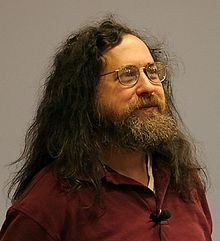
\includegraphics[height=0.27\textheight]{images/13_stallman.jpg} \hspace*{0.0cm}
		\end{center}
	  \end{flushright}
\end{frame}

\subsection{Referencias}
\begin{frame}
  \frametitle{Referencias}
    \begin{thebibliography}{10}

    \beamertemplatearticlebibitems

    \bibitem{org}
      Manjaro Linux
      \newblock {\tt http://manjaro.org}

    \bibitem{arch}
      Arch Linux
      \newblock {\tt https://www.archlinux.org/}

    \bibitem{other}
      Arch compared to other distributions
      \newblock {\tt https://wiki.archlinux.org/index.php/Arch\_compared\_\ \\to\_other\_distributions}

    \bibitem{wssblog}
      Diego Salinas Blog
      \newblock {\tt http://walkingsources.blogspot.com}

    \end{thebibliography}
\end{frame}

\subsection{...}
\begin{frame}
  \frametitle{...}
  \ \\ \ \\
  \huge Preguntas ?

  \begin{flushright}
    \ \\
    \huge Diego Salinas

    \structure{\footnotesize{dsalinas.fsd6@gmail.com}}
  \end{flushright}
\end{frame}

\end{document}
